%=======================+=========================
%================  Controls  ================
%=================================================

\section[Slow controls]{Slow controls \label{sec:controls}}
As any modern sophisticated particle detector system, \gx{} requires being able to monitor 
and control tens of thousands of different variables that define the state of the experimental hardware. Different variable values need to be acquired, displayed, archived, and used as inputs to control loops continually with a high degree of reliability. For \gx~ we archive approximately 90,000 variables, and monitor many more.

\subsection{Architecture \label{sec:controlsarchitechture}}
The \gx{} slow control system consists of three layers. The first layer consists of the remote units such as high voltage or low voltage power chassis, magnet power supplies, temperature controller, LabView applications, Programmable Logic Controller or PLC-based applications, which directly interact with the hardware and contain almost all of the control loops. The second layer is the Supervisory Control and Data Acquisition (SCADA) layer which is implemented in the form of approximately 140 EPICS\footnote{https://epics.anl.gov.} Input/Output Controllers or (IOC's). This layer provides the the interface between the low level application and the higher level applications using EPICS ChannelAccess protocol. The highest level, referred as Experiment Control System (ECS), contains the application such as Human-Machine Interface (HMI), the alarm system and data archiving. This structure allows for relatively easy and seamless addition and integration of new components into the overall controls system of \gx{}.    

\subsection{Remote Units \label{sec:controlsinterface}}
\gx{} uses a variety of commercial units that provide us with control over the hardware used in the experiment. For instance most of the detector high voltages are provided by the CAEN SYx527 voltage mainframe\footnote{https://www.caen.it/subfamilies/mainframes/} while the low and bias voltages are provided by boards residing in Wiener MPOD chassis\footnote{http://www.wiener-d.com/sc/power-supplies/mpod--lvhv/mpod-crate.html}. These two power supplies types provide most of the voltage with the exception of tagger microscope and forward calorimeter where custom systems were developed which provide voltage regulation and interact with EPICS-based layer through higher level interfaces using custom protocols, see Sections.~\ref{sec:TAGM} and \ref{sec:fcal} for more details.  

There are various beam line devices that need to be moved during beam operations. We use stepper motors to move these motorized stages via Newport XPS universal multi-axis motion controller\footnote{https://www.newport.com/c/xps-universal-multi-axis-motion-controller.} that allows for execution of complex trajectories involving multiple axes. All of the stage referencing, motion profile computations and encoder-based closed-loop control occur within the controller chassis after the basic parameters such as positions and velocities are provided by the user via TCP/IP based interface to EPICS.   

While installing complex systems, such as a superconducting magnet, we have developed a custom controls system with a large number of input, outputs channels and sophisticated logic suited for the particular system. For those cases we mostly  utilized Allen-Bradley CompactLogix and ControlLogix PLC systems\footnote{https://ab.rockwellautomation.com.}. These systems are designed for industrial systems that allow for a modular design and provide high reliability and require minimal maintenance. All of the controls loops are programmed within the PLC application. These types of PLC's are interfaced with EPICS through TCP/IP EtherNet/IP proprietary protocol to allow the higher level applications access process variables served by the PLC's.  

The cryogenic target and the superconducting solenoid magnet of \gx{} use National Instruments LabView applications. The controls of the target are done using custom-made and vendor-supplied hardware that include built-in remotely accessible control systems and a NI CompactRIO\footnote{https://www.ni.com/en-us/shop/compactrio.html} chassis that communicates with the hardware and serves the variables using internal ChannelAccess server and an EPICS IOC running on the CompactRIO controller, as described in details in Sec~\ref{sec:target}. We also use a National Instruments PXI high performance system\footnote{https://www.ni.com/en-us/shop/pxi.html} to collect data from different sensors as described in Sec.~\ref{sec:solenoid}. 

%\begin{landscape}
 \begin{figure}[p]
\begin{center}
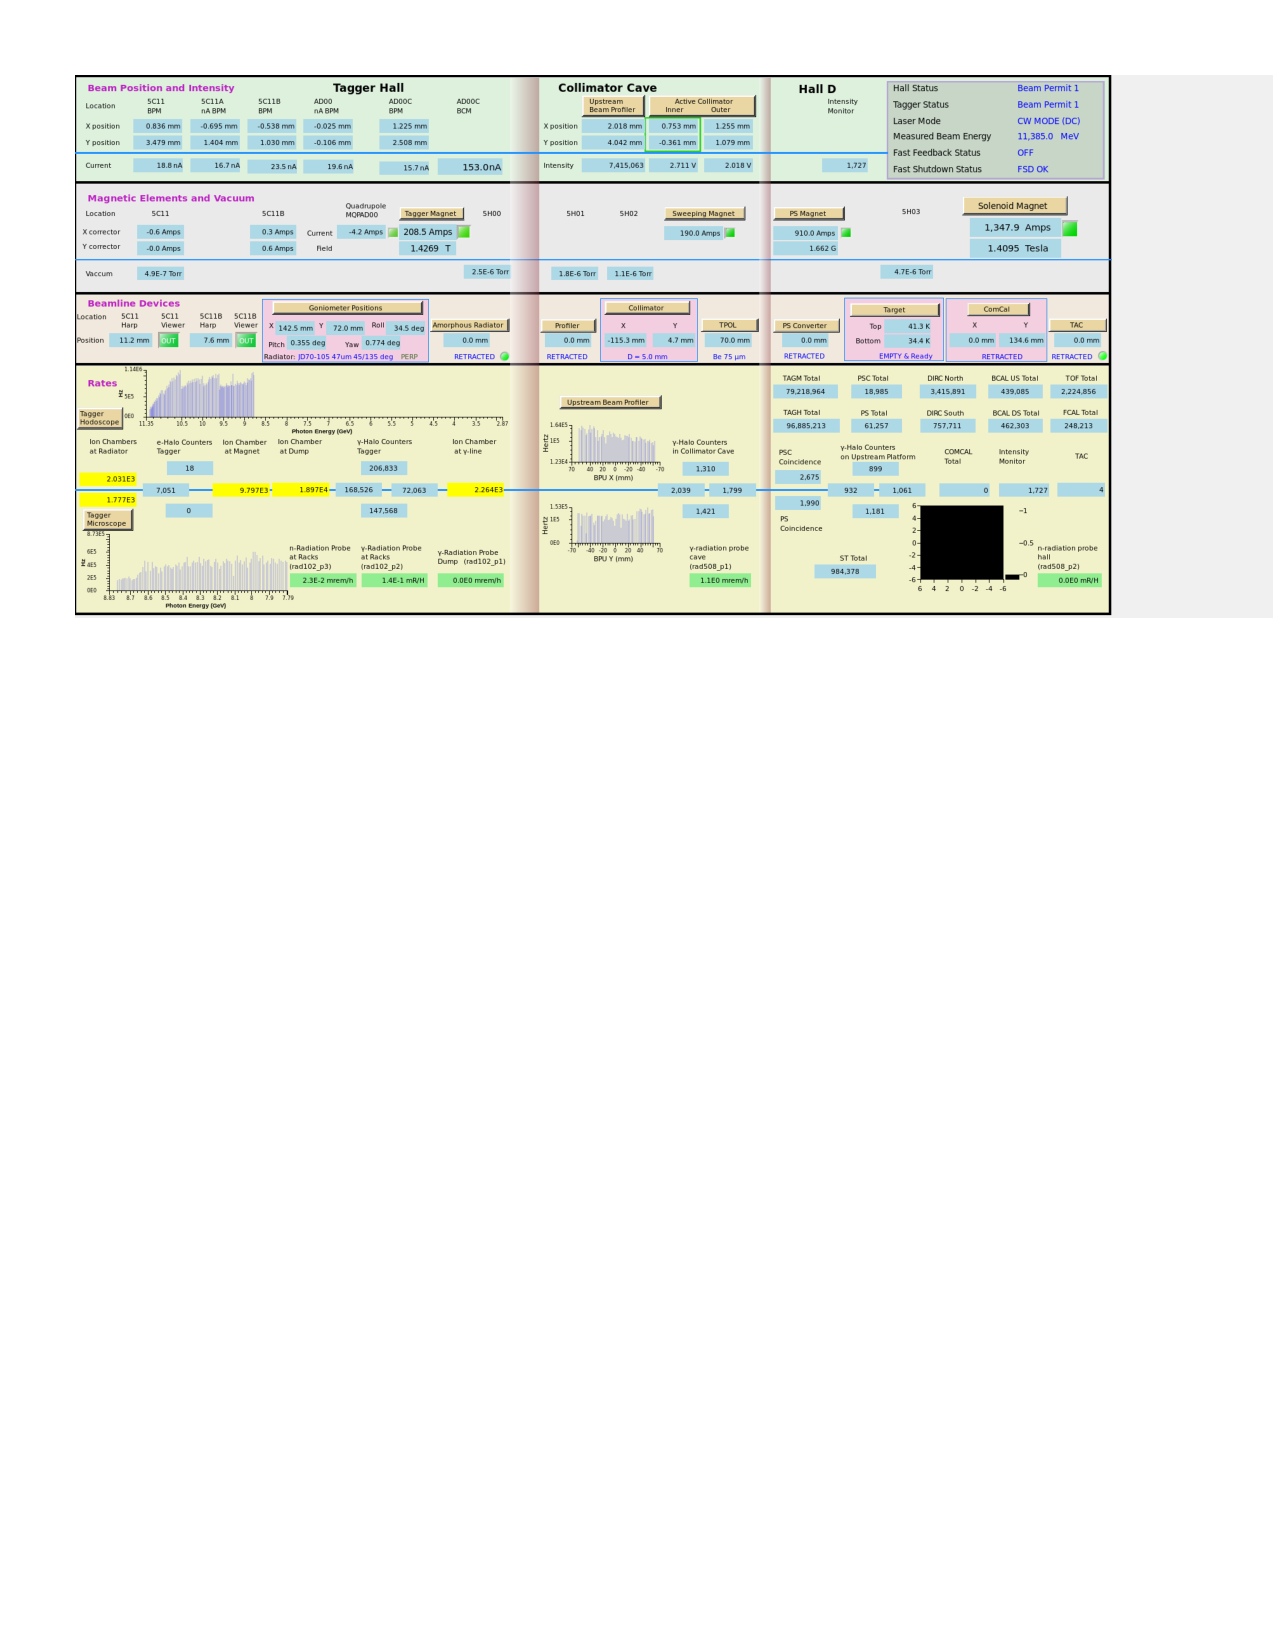
\includegraphics[height=15cm,clip=true]{figures/GlueX_CSS_overview.pdf}
\caption{Top-level graphical interface for the beamline. This screen provides information on beam currents and rates, radiators, magnet status, target condition, background levels, etc.
\label{fig:GlueX_CSS_overview}
}
\end{center}
\end{figure}
%\end{landscape}

\subsection{Supervisory Control and Data Acquisition layer \label{sec:archiver}}
The Supervisory Control and Data Acquisition (SCADA) layer is the middle layer that distributes the process variables allowing the higher level, and sometimes lower level, applications to use various process variables of Hall D controls system. This layer is based on EPICS and uses ChannelAccess protocol to publish the values of the variables over Ethernet. And because the accelerator controls also uses EPICS, this allows us to efficiently exchange the information between the experiment and the accelerator operations. There are a few dozens of software Input/Out Controller (IOC) processes running on the hosts in the experiment control room that collect the data from different components of the lowest layer. Each of these IOC's is configured to be able to communicate using the protocol appropriate for the remote units from which it needs to exchange data. For instance the EPICS IOC controlling the voltage for the FDC detector needs to be able to communicate with Wiener MPOD and CAEN SYx527 voltage chassis. Although the middle layer is there mostly to distribute the data between different applications it also contains some EPICS-based applications running on IOC's that provide different control loops and software interlocks.  For instance, the low voltage power supplies for the FDC detector (see Sec. \ref{sec:fdc}) are shut off if the temperature or the flow of the coolant in the chiller falls out of required limits. 
\subsection{Experiment Control System \label{sec:alarms}}
The highest level of controls contains the applications that archive the data, display data in interactive GUIs and as stripcharts, alarm and notify shift personnel and experts in case problems occur, and also allow for interfacing with the CODA-based data acquisition system of \gx{} described is Sec.~\ref{sec:daq}.
An example of a GUI is provided by the beamline overview screen, which shown in Fig.\,\ref{fig:GlueX_CSS_overview}. Many of the buttons are active and allow access to other GUIs.
The display management and the alarm system for \gx{} controls is based on Controls System Studio (CSS)\footnote{http://controlsystemstudio.org/}  which is an Eclipse-based toolkit for operating large systems and it is well suited for systems that use EPICS as its integral part. Although CSS provides its own archiving engine and stripcharting tools we utilized the MYA archiver~\cite{Slominski:2009icaleps} provided by the JLAB accelerator software group with its tools for displaying the archived data as time-series. The display management for \gx{} controls is done within CSS BOY~\cite{Chen:2011icaleps} environment that allows the system expert to build sophisticated control screen using standard widgets. The alarm system is based on CSS BEAST\cite{Kasemir:2009icaleps} alarm handler software which alerts the shift personnel about the problems with the detector and it also notifies the system expert if the problems are not resolved by the shift personnel in the experiments control room. 